\documentclass[tikz,border=8pt]{standalone}
\usepackage{amsmath,amssymb}
\usetikzlibrary{arrows.meta,automata,positioning,quotes}
\begin{document}
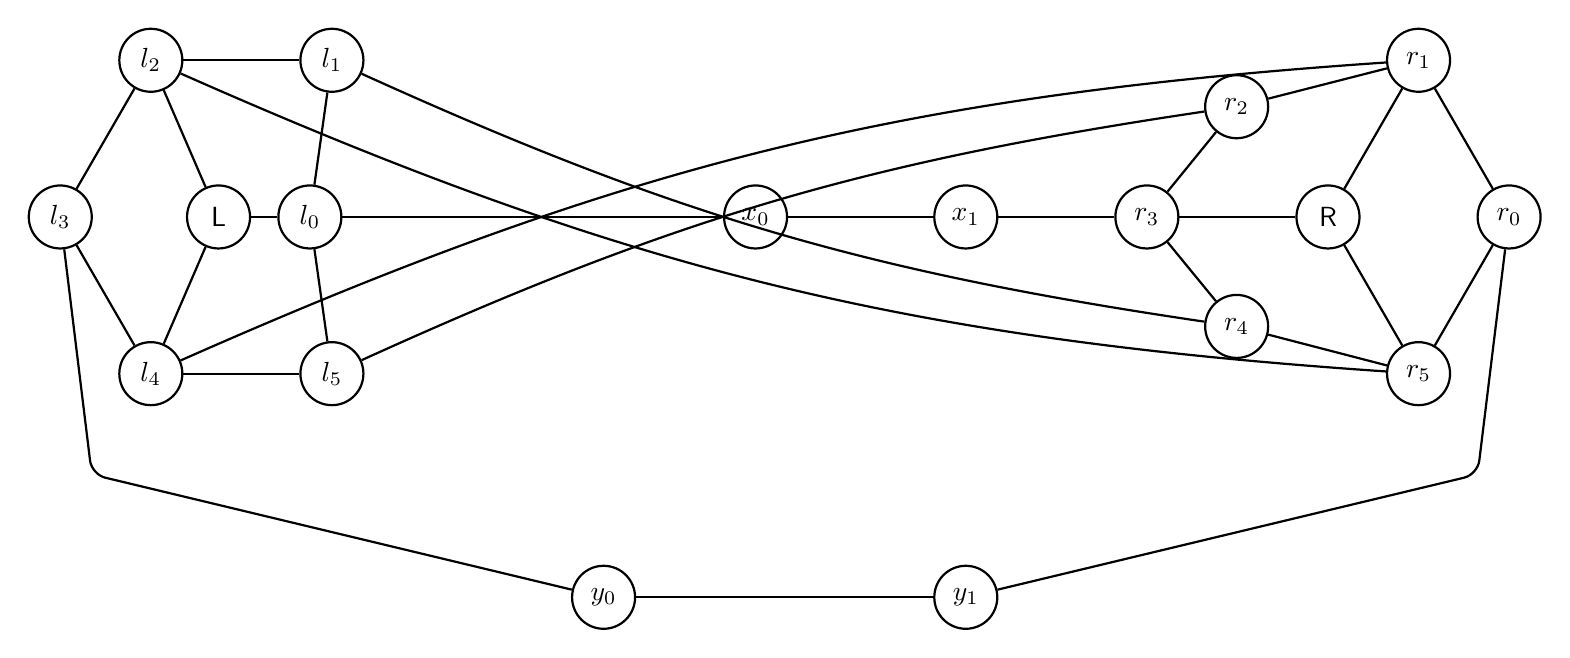
\begin{tikzpicture}[x=1cm,y=1cm]
\tikzset{
  graphnode/.style={circle,draw,thick,minimum size=8mm,inner sep=1pt,font=\sffamily},
  directed/.style={-{Stealth[length=2.4mm]},thick},
  undirected/.style={thick}
}
\node[graphnode] (n_L) at (-7.19,0.07) {L};
\node[graphnode] (n_l0) at (-6.03,0.07) {$l_{0}$};
\node[graphnode] (n_l1) at (-5.75,2.06) {$l_{1}$};
\node[graphnode] (n_l2) at (-8.05,2.06) {$l_{2}$};
\node[graphnode] (n_l3) at (-9.20,0.07) {$l_{3}$};
\node[graphnode] (n_l4) at (-8.05,-1.92) {$l_{4}$};
\node[graphnode] (n_l5) at (-5.75,-1.92) {$l_{5}$};
\node[graphnode] (n_R) at (6.90,0.07) {R};
\node[graphnode] (n_r0) at (9.20,0.07) {$r_{0}$};
\node[graphnode] (n_r1) at (8.05,2.06) {$r_{1}$};
\node[graphnode] (n_r2) at (5.74,1.47) {$r_{2}$};
\node[graphnode] (n_r3) at (4.60,0.07) {$r_{3}$};
\node[graphnode] (n_r4) at (5.74,-1.32) {$r_{4}$};
\node[graphnode] (n_r5) at (8.05,-1.92) {$r_{5}$};
\node[graphnode] (n_x0) at (-0.37,0.07) {$x_{0}$};
\node[graphnode] (n_x1) at (2.30,0.07) {$x_{1}$};
\node[graphnode] (n_y0) at (-2.30,-4.76) {$y_{0}$};
\node[graphnode] (n_y1) at (2.30,-4.76) {$y_{1}$};
\draw[undirected] (n_l0) -- (n_l1);
\draw[undirected] (n_l1) -- (n_l2);
\draw[undirected] (n_l2) -- (n_l3);
\draw[undirected] (n_l3) -- (n_l4);
\draw[undirected] (n_l4) -- (n_l5);
\draw[undirected] (n_l5) -- (n_l0);
\draw[undirected] (n_L) -- (n_l0);
\draw[undirected] (n_L) -- (n_l2);
\draw[undirected] (n_L) -- (n_l4);
\draw[undirected] (n_r0) -- (n_r1);
\draw[undirected] (n_r1) -- (n_r2);
\draw[undirected] (n_r2) -- (n_r3);
\draw[undirected] (n_r3) -- (n_r4);
\draw[undirected] (n_r4) -- (n_r5);
\draw[undirected] (n_r5) -- (n_r0);
\draw[undirected] (n_R) -- (n_r1);
\draw[undirected] (n_R) -- (n_r3);
\draw[undirected] (n_R) -- (n_r5);
\draw[undirected] (n_l0) -- (n_x0);
\draw[undirected] (n_x0) -- (n_x1);
\draw[undirected] (n_x1) -- (n_r3);
\draw[undirected,rounded corners=5pt] (n_l3) -- (-8.80,-3.20) -- (n_y0);
\draw[undirected] (n_y0) -- (n_y1);
\draw[undirected,rounded corners=5pt] (n_y1) -- (8.80,-3.20) -- (n_r0);
\draw[undirected] (n_l1) to[bend right=8] (n_r4);
\draw[undirected] (n_l2) to[bend right=10] (n_r5);
\draw[undirected] (n_l4) to[bend left=10] (n_r1);
\draw[undirected] (n_l5) to[bend left=8] (n_r2);
\end{tikzpicture}
\end{document}
